\section{Resultados}
Se obtuvo Neuralyrics, una aplicación web con inteligencia artificial en línea funcional para la generación de nuevas letras musicales del género pop con la intención de ayudar a artistas en necesidad de ideas para generar nuevas canciones, así como un modelo entrenado con el 2.5\% del dataset original. El algoritmo para llamar al modelo consta de dos elementos esenciales para generar la letra: estructura y semántica.\\\\
Se evaluó al algoritmo usando la precisión que arrojó el modelo que fue de un 58\%, esto indica que por cada palabra que se predice, hay una probabilidad muy alta de que sea muy parecida a otra canción existente, dato que nos señala la probabilidad de que con un modelo entrenado con más canciones pueda tener una precisión más baja y pueda generar textos variados y con una semántica correcta. Igualmente se obtuvieron registros de las interacciones de los usuarios en la página web, los cuales nos permiten analizar las partes que fueron relevantes y cuánto impacto se tiene en el internet.
\begin{figure}[h]
	\centering
	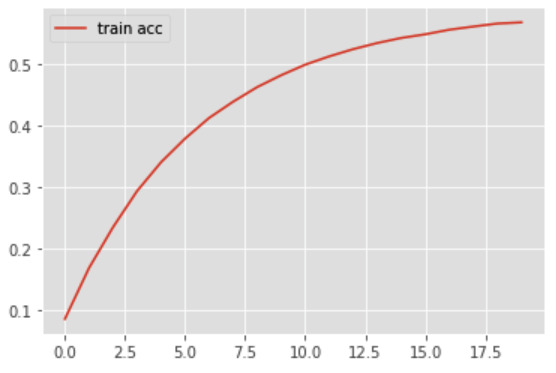
\includegraphics[width=8cm]{figuras/Graficapre.png}
	\caption{Gráfica sobre la presición del modelo}
	\label{fig:Gráfica sobre la presición del modelo}
\end{figure}
\subsection{Demostración online}
Una demostración online para la generación de letras musicales se encuentra disponible en neuralyrics.com, y fue creada con la intención de:
\begin{enumerate}
    \item Poner el generador a disposición del público.
    \item Proporcionar a los usuarios formas fáciles de personalizar las letras generadas.
    \item Recopile registros de uso limitado para evaluar y mejorar el algoritmo.
\end{enumerate}
El sitio web se lanzó en noviembre del 2021.